\qrchapter{https://forgottenpillar.com/rsc/pl-fp-chapter10}{Czy Bóg jest osobą? — John N. Loughborough}

Jeden z najwcześniejszych artykułów na temat \emcap{osobowości Boga} to artykuł Loughborougha „\textit{Czy Bóg jest osobą?}”, w którym omawia \emcap{osobowość Boga} i Jego obecność. Ważne jest, aby pamiętać definicję ‘osobowości’ według słownika Merriam-Webster: „\textit{właściwość lub stan jako osoby}”\footnote{\href{https://www.merriam-webster.com/dictionary/personality}{Merriam-Webster Dictionary — ‘\textit{personality}’.}}. Przyjrzymy się uważnie, jak Loughborough postrzega właściwość lub stan Boga jako osoby.

\begin{figure}[hp]
    \centering
    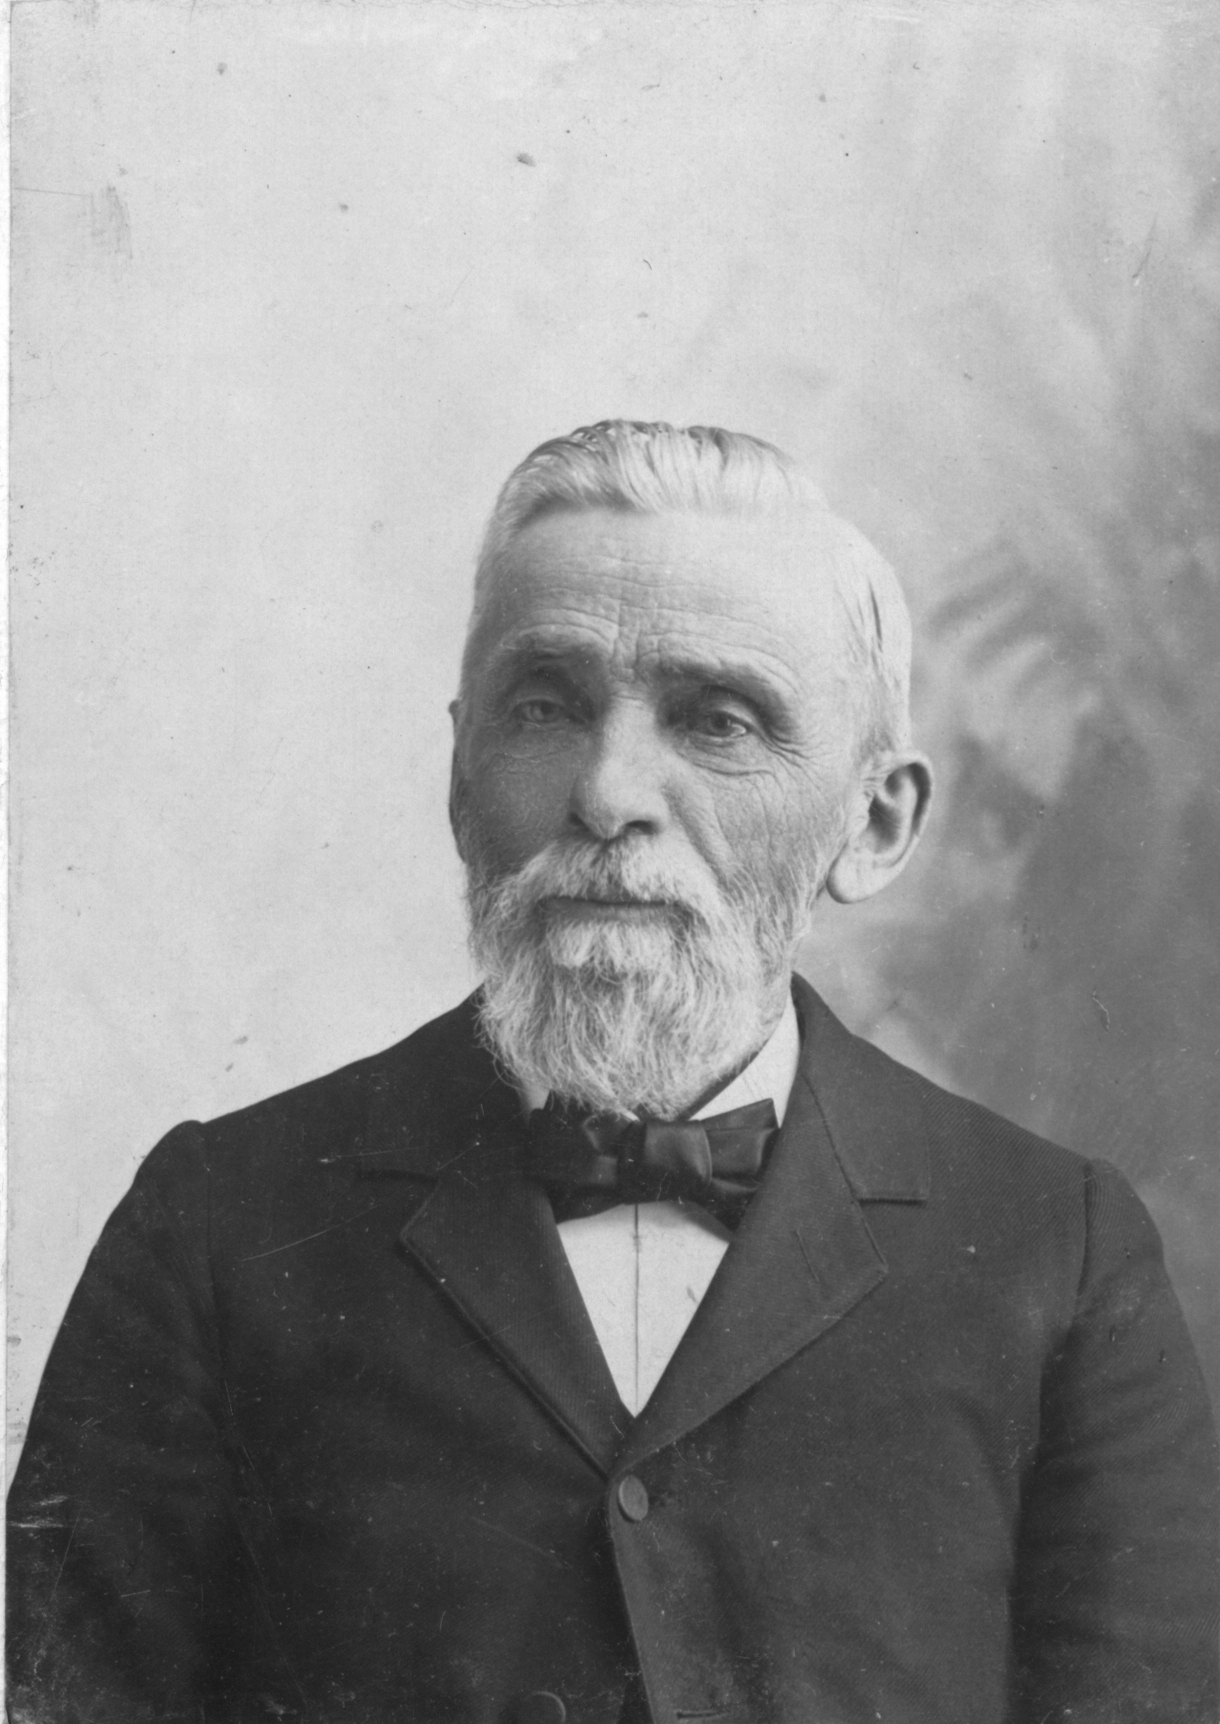
\includegraphics[width=1\linewidth]{images/john-n-loughborough.jpg}
    \caption*{John Norton Loughborough (1832-1924)}
    \label{fig:john-n-loughborough}
\end{figure}

\othersnogap{Jakakolwiek może być prawda w tej sprawie, z pewnością nie może być błędem zbadanie tego, co mówi na ten temat Słowo. \textbf{Jest wielu takich, którzy powstrzymują się od badania niepopularnych prawd, ponieważ podnosi się przeciwko nim krzyk o herezję}. Nie będziemy uważać się za podmioty tego określenia \textbf{ani nie wnikamy w tajemnice Wszechmogącego, gdy prowadzimy badanie tej sprawy}. Biblia z pewnością zawiera świadectwo w tej kwestii i, powtarzamy ponownie: «\textbf{Rzeczy, które są objawione, należą do nas}». Pytamy więc: Co mówi Pismo?}

\othersnogap{\textbf{To samo świadectwo, które badaliśmy odnośnie do stworzenia człowieka z prochu \underline{na obraz Boga}, dowodzi jednoznacznie, że \underline{Bóg ma postać}, chociaż ten pogląd jest sprzeczny z tym, czego uczono nas jako dzieci z katechizmu}:}

\othersnogap{«Pytanie: Czym jest Bóg?»}

\othersnogap{«Odpowiedź: Nieskończonym i wiecznym duchem; tym, który zawsze był i zawsze będzie»}

\othersnogap{«Pyt.: Gdzie jest Bóg?»}

\othersnogap{«Odp.: Wszędzie»}

\othersnogap{\textbf{Lecz pytamy: \underline{Czy Bóg nie jest w jednym miejscu bardziej niż w innym}?} Och nie, mówicie: \textbf{Biblia mówi, że \underline{jest duchem}, a jeśli tak, to musi być \underline{wszędzie tak samo}}. Cóż, jeśli w momencie śmierci człowieka jego duch idzie do Boga, to musi iść wszędzie. \textbf{Lecz Biblia niewątpliwie przedstawia Boga jako umiejscowionego w niebie. «Spojrzał bowiem w dół z wysokości swojego przybytku; z nieba Pan popatrzył na ziemię». Ps 102:19}. \textbf{Zatem z pewnością niebo nie może być wszędzie, ponieważ Bóg jest przedstawiony jako spoglądający z niego. «\underline{Eliasz wstąpił} wśród wichru \underline{do nieba}». 2Krl 2:11}. \textbf{Ale, ktoś powie, czy Biblia nie przedstawia Boga jako \underline{wszechobecnego}?} Ps 139:8--10. «Jeśli wstąpię do nieba, \textbf{jesteś tam}; jeśli przygotuję sobie posłanie w piekle, \textbf{oto tam jesteś}; gdybym wziął skrzydła poranka i zamieszkał na krańcu morza, \textbf{i tam twoja ręka prowadziłaby mnie}, a twoja prawica by mnie podtrzymała»}

\othersnogap{Odpowiadamy — \textbf{temat jest wprowadzony w wersecie 7 następująco}: «\textbf{\underline{Dokąd ujdę przed twoim Duchem}?} \textbf{Albo dokąd ucieknę przed \underline{twoją obecnością}?}» \textbf{Duch jest \underline{przedstawicielem Boga}}. \textbf{Jego moc objawia się wszędzie tam, gdzie zechce, poprzez działanie Jego Ducha}. Chrystus, dając uczniom zlecenie, mówi: «Idźcie na cały świat i głoście ewangelię wszelkiemu stworzeniu, a oto \textbf{ja jestem z wami przez wszystkie dni aż do końca świata}». Otóż nikt nie będzie twierdził, że Chrystus był osobiście na ziemi przez cały czas od momentu, gdy uczniowie zaczęli wypełniać to zlecenie. \textbf{Ale Jego Duch był na ziemi; Pocieszyciel, którego obiecał posłać.} \textbf{W ten sam sposób Bóg objawia się \underline{przez swojego Ducha}, który jest również mocą, przez którą działa}. «Lecz jeśli \textbf{Duch tego}, który wskrzesił Jezusa z martwych, mieszka w was, \textbf{ten, który wskrzesił} Chrystusa z martwych, ożywi też wasze śmiertelne ciała \textbf{\underline{przez swego Ducha}, który w was mieszka}». Rz 8:11. \textbf{\underline{Jest tu wyraźne rozróżnienie między Duchem a Bogiem, który wskrzesza umarłych przez tego Ducha}}. \textbf{Jeśli żywy Bóg jest Duchem w najściślejszym znaczeniu tego słowa, a jednocześnie posiada Ducha, to mamy od razu nowatorską ideę Ducha Ducha, do której wyjaśnienia potrzeba co najmniej spirytualisty}}[The Adventist Review and Sabbath Herald, 18 września 1855 r.][https://documents.adventistarchives.org/Periodicals/RH/RH18550918-V07-06.pdf]

Pozwól nam na krótki komentarz. Mamy nadzieję, że rozpoznajesz konkretny temat, który jest tu omawiany. Tematem jest pierwszy punkt \emcap{Fundamentalnych Zasad} i twierdzenie, że Bóg ma postać, ponieważ człowiek został stworzony na obraz Boga. Takie zrozumienie osobowości Boga wyklucza ideę, że Bóg jest wszędzie obecny. Brat Loughborough podał biblijne powody wszechobecności Boga, wraz z poglądem, że „\textit{Bóg jest w jednym miejscu bardziej niż w innym}”. Bóg jest wszędzie obecny przez swojego przedstawiciela, Ducha Świętego, tak jak jest napisane w pierwszym punkcie \emcap{Fundamentalnych Zasad}. W dalszej części tej dyskusji przeczytamy, że Bóg jest istotą duchową i posiada namacalne, materialne ciało, w przeciwieństwie do idei, że jest On wyłącznie duchem.

\others{Istnieje co najmniej jedna nieprzekraczalna trudność na drodze \textbf{tych, którzy wierzą, że \underline{Bóg jest niematerialny}, a niebo nie jest dosłownym, \underline{zlokalizowanym miejscem}: są zmuszeni przyznać, że \underline{Jezus jest tam cieleśnie, jako dosłowna osoba}}; ten sam Jezus, który został ukrzyżowany, umarł i został pogrzebany, został wskrzeszony z martwych, \textbf{wstąpił do nieba} i jest teraz \textbf{po prawicy Boga}. \textbf{Jezus posiadał ciało i kości po swoim zmartwychwstaniu}. Łk 24:39. «\textbf{Popatrzcie na moje dłonie i stopy, że to jestem ja sam; dotknijcie mnie i zobaczcie; \underline{bo duch nie ma ciała ani kości, jak widzicie, że ja mam}}». \textbf{Jeżeli Jezus jest tam w niebie z dosłownym ciałem i dosłownymi kośćmi, czy niebo nie może być jednak dosłownym miejscem, mieszkaniem dla dosłownego Boga, dosłownego Zbawiciela, dosłownych aniołów i zmartwychwstałych nieśmiertelnych świętych?} \textbf{\underline{O nie, powie ktoś: «Bóg jest Duchem».}} Tak Chrystus powiedział do kobiety z Samarii przy studni. \textbf{Nie jest konieczny wniosek, że skoro Bóg jest Duchem, \underline{to nie ma ciała}}. W J 3:6 Chrystus mówi do Nikodema: «\textbf{Co się narodziło z Ducha, jest duchem}». \textbf{Jeśli to, co narodziło się z Ducha, jest duchem, to na tej samej zasadzie to, co ma duchową naturę, jest duchem. Bóg jest \underline{istotą duchową}, Jego natura jest duchem, nie jest On śmiertelnej natury;} \textbf{\underline{ale to nie wyklucza idei, że ma On ciało}}. Dawid mówi [Ps 104:4]: «Który czyni \textbf{swoich aniołów duchami}»; jednak \textbf{\underline{aniołowie mają ciała}}. Aniołowie ukazali się zarówno Abrahamowi, jak i Lotowi i jedli z nimi. \textbf{Widzimy, że idea, iż aniołowie są duchami, nie dowodzi, że nie są oni dosłownymi istotami}}

\othersnogap{Sugeruje się, że ponieważ Biblia mówi, że Bóg jest Duchem, to nie jest On osobą. Sugestia nie powinna być podstawą argumentu. Wielkie prawdy Pisma są jasno określone i nie możemy opierać doktryny na sugestiach \textbf{sprzecznych ze stanowczymi stwierdzeniami w Słowie Bożym}. Jeśli Pismo stwierdza w stanowczych \textbf{słowach, że Bóg jest osobą, nie możemy wyciągać wniosku z tekstu, który mówi: «Bóg jest Duchem», \underline{że nie ma On ciała}}}

\othersnogap{Przedstawimy teraz kilka tekstów, które \textbf{dowodzą, że Bóg jest osobą}. Wj 33:18, 23. «I (Mojżesz) powiedział: Proszę cię, ukaż mi swoją chwałę». Werset 20. «I powiedział: \textbf{Nie możesz zobaczyć \underline{mego oblicza}, bo człowiek nie może ujrzeć mnie i przeżyć}». Wersety 21--23. «I Pan rzekł: Oto miejsce przy mnie, a ty staniesz na skale; i stanie się, gdy będzie przechodzić moja chwała, że postawię cię w rozpadlinie skalnej i \textbf{zakryję cię \underline{swoją ręką}, kiedy będę przechodził}; potem odejmę \textbf{swoją rękę} i \textbf{ujrzysz moje \underline{plecy}}; lecz \textbf{\underline{moje oblicze} nie będzie widziane}». \textbf{Jeśli Bóg jest \underline{niematerialnym Duchem}, to Mojżesz nie mógłby Go zobaczyć, ponieważ mówi się nam, że duch nie może być widziany zwykłymi oczami}. \textbf{Nie byłoby wtedy sensu, aby Bóg mówił, że położy swoją rękę na twarzy Mojżesza, gdy będzie przechodził (najwyraźniej, aby uniemożliwić mu zobaczenie Jego oblicza), ponieważ i tak nie mógłby Go zobaczyć}. Nie wyobrażamy sobie też, jak niematerialna ręka mogłaby powstrzymać promienie światła przed dotarciem do oczu Mojżesza. \textbf{Ale jeśli stanowisko, \underline{że Bóg jest niematerialny} i nie może być widziany zwykłym okiem, jest prawdziwe, powyższy tekst jest całkowicie zbędny}. \textbf{Jaki jest sens w mówieniu, że Bóg położył swoją rękę na twarzy Mojżesza, aby uniemożliwić mu zobaczenie tego, czego i tak nie można zobaczyć?}}

\othersnogap{Ktoś powie: Widzę, że nie możemy zharmonizować tej sprawy w inny sposób, niż że Mojżesz widział dosłowne ciało; ale to nie było własne ciało Boga, \textbf{lecz było ciało, które przyjął, aby pokazać się Mojżeszowi}. \textbf{Mojżesz nie mógłby właściwie pojąć Boga, gdyby Ten nie przyjął postaci}. \textbf{Zatem Bóg przyjął ciało}. To rzuca gorsze światło na sprawę niż pierwsze stanowisko; \textbf{ponieważ oskarża o zwiedzenie Boga, który mówiłby Mojżeszowi, że zobaczy Jego, podczas gdy w rzeczywistości Mojżesz według tego świadectwa nie widział Boga, ale inne ciało}. Człowiek musiałby być prawie beznadziejnie pogrążony w wątpliwościach, aby próbować w ten sposób mistyfikować i niwelować siłę tego świadectwa}[Tamże.][https://documents.adventistarchives.org/Periodicals/RH/RH18550918-V07-06.pdf]

Czy rozpoznajecie, że brat Loughborough zajmuje się poglądem, który dr Kellogg przedstawi w \textit{The Living Temple} 48 lat później? Dr Kellogg powiedział, że to prawda, że Bóg przedstawił się w \othersnodot{\textbf{\underline{konkretnej postaci lub konkretnym miejscu}}}[John H. Kellogg, The Living Temple, str. 31.][https://archive.org/details/J.H.Kellogg.TheLivingTemple1903/page/n31/], ponieważ \others{musi być coś bardziej \textbf{namacalnego}, bardziej \textbf{\underline{ograniczonego}}, na czym można skupić umysł w uwielbieniu}[Tamże, str. 30.][https://archive.org/details/J.H.Kellogg.TheLivingTemple1903/page/n30/], ale że w rzeczywistości jest On \othersnodot{\textbf{daleko poza naszym zrozumieniem \underline{jak granice przestrzeni i czasu}}}[Tamże, str. 33.][https://archive.org/details/J.H.Kellogg.TheLivingTemple1903/page/n33/]. Brat Loughborough słusznie sprzeciwił się idei, że Bóg tylko objawia się człowiekowi jako określona Istota, ale w rzeczywistości nie jest tym, za kogo się podaje. Takie twierdzenie \othersnodot{oskarża Boga o zwiedzenie}. Brat Loughborough kontynuuje z twierdzącym, biblijnym świadectwem, że Bóg jest istotą materialną.

\others{Wj 24:9. «I wstąpili Mojżesz, Aaron, Nadab i Abihu oraz siedemdziesięciu ze starszych Izraela, \textbf{i widzieli Boga Izraela}: a pod \textbf{jego nogami} było jakby dzieło z szafirowego kamienia jak niebo w swej jasności». Pozwolono im \textbf{zobaczyć Jego nogi}, ale żaden \textbf{człowiek nie może widzieć Jego oblicza i przeżyć}. \textbf{Żadne \underline{śmiertelne oko} nie może znieść olśniewającej jasności tej chwały oblicza Boga}. Znacznie przewyższa ona światło słońca. Prorok bowiem mówi: «Światło księżyca będzie jak światło słońca, światło słońca będzie \textbf{siedmiokrotnie jaśniejsze}, jakby światło siedmiu dni, w dniu, kiedy Pan obwiąże złamanie swego ludu i uleczy zadaną mu ranę». Iz 30:26. Mimo tego siedmiokrotnego światła, które wtedy będzie świecić, prorok, mówiąc o tej scenie, powiada: «Wtedy księżyc zarumieni się i słońce się zawstydzi, gdy Pan zastępów będzie królował na górze Syjon i w Jerozolimie, i wobec swoich starszych w chwale». Iz 24:23. Świadectwo Jana brzmi [Obj 21:23]: «A miasto nie potrzebowało słońca ani księżyca, aby świeciły w nim, bo \textbf{chwała Boga je oświetlała}, a Baranek jest jego lampą».}

\othersnogap{\textbf{Niewierzący twierdzą, że istnieje sprzeczność w świadectwie Mojżesza, ponieważ powiedział, że rozmawiał z Bogiem twarzą w twarz}. \textbf{Odpowiadamy, że była między nimi chmura}, ale Bóg powiedział Mojżeszowi: «\textbf{Człowiek nie może ujrzeć mnie i przeżyć}». Świadectwo Nowego Testamentu jest zgodne ze Starym w tej kwestii. «Dążcie do pokoju ze wszystkimi ludźmi, i do świętości, bez której \textbf{nikt nie ujrzy Pana}». Hbr 12:14. \textbf{Kto \underline{śmiertelnymi oczami} mógłby patrzeć na światło, które siedmiokrotnie przewyższa jasność słońca?} Z pewnością tylko święci mogą Go oglądać, \textbf{tylko nieśmiertelne oczy} mogłyby znieść tę promienną chwałę. Chociaż Słowo mówi, że nie możemy teraz ujrzeć Boga i przeżyć, obietnica głosi, że \textbf{czystego serca ujrzą Go}. Mt 5:8. «Błogosławieni czystego serca, \textbf{ponieważ oni zobaczą Boga}». Obj 22:4. «I \textbf{będą oglądać Jego oblicze}, a Jego imię będzie na ich czołach».}

\othersnogap{Paweł [Kol 1:15], wypowiadając się o Chrystusie, mówi: «On jest obrazem \textbf{niewidzialnego Boga}, pierworodnym wszelkiego stworzenia». Tutaj Chrystus jest nazwany «\textbf{obrazem niewidzialnego Boga}». Już pokazaliśmy, że \textbf{Chrystus składa się z substancji, ciała i kości; i jest nazwany} «\textbf{obrazem niewidzialnego Boga}». No cóż, powie ktoś, przyznajemy, że Jego boska natura jest na obraz Boga. Jeżeli przez Jego boską naturę rozumie się część, która istniała w chwale z Ojcem przed powstaniem świata, odpowiadamy, że to, co było na początku u Boga (Słowo), \textbf{stało się ciałem, nie weszło w ciało}, lub jak niektórzy twierdzą, \textbf{przyodziało się w ludzką naturę, ale stało się ciałem}. Lecz ktoś inny powie: \textbf{Bóg jest nazwany niewidzialnym}. \textbf{To, że jest On teraz niewidzialny, nie dowodzi, że nigdy nie będzie widziany}. Słowo mówi: «Czystego serca \textbf{zobaczą Go}». Ochocza wiara mówi: Amen.}

\othersnogap{Świadectwo w Flp 2:5--6 jasno pokazuje, co można rozumieć przez stwierdzenie, że Chrystus jest obrazem Boga. «Niech będzie w was takie nastawienie umysłu, jakie też było w Chrystusie Jezusie, który \textbf{będąc w postaci Boga}, nie uważał \textbf{bycia równym Bogu} za grabież». \textbf{Jak można powiedzieć, że Chrystus jest w postaci Boga, jeśli Bóg nie ma postaci?} Rz 8:3. «Bóg, posławszy swego Syna w podobieństwie grzesznego ciała». \textbf{Chrystus jest w postaci Boga i w postaci człowieka. To od razu objawia nam postać Boga}}

\othersnogap{\textbf{\underline{Daniel, mówiąc o Bogu, nazywa Go Odwiecznym}}. Dn 7:9. «A Odwieczny zasiadł, \textbf{którego szata była biała jak śnieg}, a \textbf{włosy jego głowy} jak czysta wełna». \textbf{O tej osobie powiedziano, że ma głowę i włosy; z pewnością nie można by tego powiedzieć} \textbf{\underline{gdyby był niematerialny i nie miał postaci}}. \textbf{Lecz świadectwo Pawła w \underline{Hbr 1:3} powinno rozstrzygnąć w każdym szczerym umyśle \underline{kwestię osobowości Boga}}. Wypowiadając się o Chrystusie, mówi: «Który, będąc blaskiem Jego chwały \textbf{i dokładnym obrazem jego (to jest \underline{Ojca}) osoby}». \textbf{Tutaj jest wyraźnie stwierdzone, że \underline{Bóg ma osobowość}. Chrystus jest jej dokładnym obrazem.} Wtedy możemy zrozumieć Chrystusa, gdy mówi: «\textbf{Kto mnie widział, widzi i mego Ojca}». J 14:19. \textbf{Nie mógł mieć na myśli, że był swoim własnym ojcem; bo gdy się modlił, zwracał się do Ojca jako do innej osoby, która posłała Go na świat}. Nazywał siebie \textbf{Synem Bożym}. \textbf{Zatem nie mógł być Ojcem, którego był synem}. Kiedy mówi: «Kto mnie widzi, widzi i mego Ojca», musi mieć na myśli, że ponieważ \textbf{był dokładnym obrazem osoby Ojca, ci, którzy Go widzieli, widzieli w Nim podobieństwo Ojca}.}[The Adventist Review and Sabbath Herald, 18 września 1855 r.][https://documents.adventistarchives.org/Periodicals/RH/RH18550918-V07-06.pdf]

Ważne jest, aby zwrócić uwagę na biblijne dowody, które brat Loughborough wskazuje w świadectwie, że Bóg ma ciało. Brat Loughborough analizuje kilka fragmentów Biblii dowodzących, że Bóg rzeczywiście ma materialne ciało, ale jest ono niewidzialne dla naszych śmiertelnych oczu. Siostra White napisała to samo, gdy powiedziała: \egwinline{\textbf{Ojciec jest pełnią Bóstwa \underline{cieleśnie}} i \textbf{jest niewidzialny dla śmiertelnego wzroku}}[Ms21-1906.9; 1906][https://egwwritings.org/read?panels=p9754.16]. Żadne śmiertelne oko nie może zobaczyć Ojca, ale to nie dowodzi, że Boga nigdy nie można zobaczyć. Jezus powiedział: \bible{\textbf{Kto mnie widział, widział i mego Ojca}}[J 14:19]. Jezus wyjaśnił te słowa dwa rozdziały wcześniej: \bible{A Jezus wołał: Kto wierzy we mnie, nie we mnie wierzy, \textbf{ale w tego, który mnie posłał}. I \textbf{kto mnie widzi, widzi tego, który mnie posłał.}}[J 12:44--45]. Jezus nie posłał samego siebie, ani nie jest Jezus Ojcem, jedną i tą samą osobą; ale widzimy Ojca w Chrystusie, ponieważ On jest \textit{wyrazem istoty Ojca}. (Hbr 1:3). Jak Jezus jest osobą, posiadającą ciało, tak jest i Ojciec. Brat Loughborough kontynuuje dowodzenie swojego punktu, że Bóg jest osobą, posiadającą postać i kształt, ponieważ człowiek został stworzony na obraz Boga.

\others{A teraz powróćmy do tematu stworzenia człowieka. \textbf{Widzieliśmy już, że stworzenie człowieka na obraz Boga nie mogło odnosić się do obrazu moralnego, ponieważ oznaczałoby to absurd, że martwa glina, z której uformowany został człowiek, miała charakter jak Boga}. \textbf{Teraz widzimy, że Pisma wyraźnie uczą, że \underline{Bóg jest osobą z ciałem i postacią}}. Zatem Rdz 1:26 może być rozumiana jako nauczająca faktu, \textbf{że człowiek został stworzony na podobieństwo Boga}. Inne pisma zgadzają się z tym świadectwem. Patrz Rdz 9:6. «Kto przeleje krew człowieka, przez człowieka będzie przelana jego krew, \textbf{bo na obraz Boga człowiek został stworzony}». \textbf{\underline{To świadectwo nie może odnosić się do ducha lub niematerialnej części człowieka: to, co jest na obraz Boga, ma krew}}. 1Kor 11:7. «Mężczyzna zaś nie powinien nakrywać głowy, \textbf{gdyż jest obrazem i chwałą Boga}». Jakub [rozdz. 3:9], odnosząc się do języka mówi: «Nim błogosławimy Boga i Ojca i nim przeklinamy ludzi \textbf{stworzonych na podobieństwo (wizerunek, podobizna — Webster) Boga}». \textbf{Powyższe świadectwo rozstrzyga kwestię, \underline{że obraz Boga nie odnosi się do charakteru, ale do postaci}}.}

\othersnogap{Rdz 2:7. «\textbf{Wtedy PAN Bóg ukształtował człowieka z prochu ziemi i tchnął w jego nozdrza tchnienie życia. I człowiek stał się żywą duszą}».}[The Adventist Review and Sabbath Herald, 18 września 1855][https://documents.adventistarchives.org/Periodicals/RH/RH18550918-V07-06.pdf]

Bóg ukształtował człowieka na swój własny obraz. Bóg jest osobą, mającą ciało, kształt i postać, i ukształtował człowieka na swój własny obraz. Z tego rozumowania wyprowadzamy oczywiste znaczenie świadectwa Pisma o \emcap{osobowości Boga}. Jeśli tworzymy fałszywe koncepcje dotyczące osoby Boga, jesteśmy w niebezpieczeństwie błędnego zrozumienia innych prawd, które są związane z naturą człowieka (śmiertelność duszy, stan umarłych itd.). W swoim artykule brat Loughborough przechodzi do wyjaśniania związku między fałszywą doktryną o nieśmiertelności duszy a błędnymi koncepcjami dotyczącymi \emcap{osobowości Boga}. Jego artykuł w Review and Herald 18 września został zaczerpnięty z jego książki \textit{An Examination of the Scripture Testimony}\footnote{\href{https://egwwritings.org/?ref=en_MPC.2&para=961.2}{John Norton Loughborough, An Examination of the Scripture Testimony, 1855}}.

\begin{titledpoem}

    \stanza{
        Wysoko w niebie, na swoim tronie, \\
        Zasiada Ojciec w swojej koronie. \\
        Istota to jest całkiem realna, \\
        Choć dla naszych oczu — niewidzialna.
    }

    \stanza{
        A Boża chwała zbyt jasno świeci, \\
        By mogły widzieć ją ziemskie dzieci. \\
        Lecz mimo wszystko przez Ducha swego \\
        Bóg nam posyła obecność Jego.
    }

    \stanza{
        A w Synu obraz Ojca jest cały, \\
        W sposób odbija Go doskonały. \\
        I w Synu łaskę Ojca widzimy, \\
        Tak że za twarzą Jego tęsknimy.
    }

    \stanza{
        On z prochu ziemi nas ukształtował, \\
        Jak wcześniej z Ojcem swym zaplanował. \\
        Był na kształt Boga Adam stworzony, \\
        Nie tylko w cechach upodobniony.
    }

    \stanza{
        Osoba, co ma ciało prawdziwe, \\
        Nie mgła bezkształtna — zdanie fałszywe. \\
        Ojciec czeka, choć nie widzi oko, \\
        Aż czyste serca wzlecą wysoko.
    }

\end{titledpoem}

